\chapter{Theoretical Framework}
\lhead{Chapter 2 \emph{Theoretical Framework}}
\label{chap:2}
%\autoref{chap:2}

\section{The space environment capacity mechanisms}
\bigskip

Near-Earth space is a finite and an inherently %=έμφυτα, εγγενώς
international natural resource. At the same time, there is no ownership in space, as it is stated by UNOOSA in the Outer Space Treaty. However, it seems that nowadays it can be linked to the phenomenon of Tragedy of Commons written by the British economist Lloyd \cite{Wang}. Based on this concept, the shared-resource system is spoiled by individual users who act based on their own benefit and against the common good. This notion describes the current situation of the space industry, which comes as an international problem.

\bigskip
The source and sink mechanisms, which can explain how the numbers of objects orbiting Earth have increased, were described by Somma et al. [2018]. This aforementioned work \cite{Somma 2019} presents the equations of the injection and removal of an object from any altitude range from 200 to 2000 km. As it can be seen in Figure \ref{mechanism}, new objects are created by launches, explosions and collisions. Conversely, an object can be removed due to natural drag, post-mission disposal, and active debris removal.

\begin{figure}
\centering
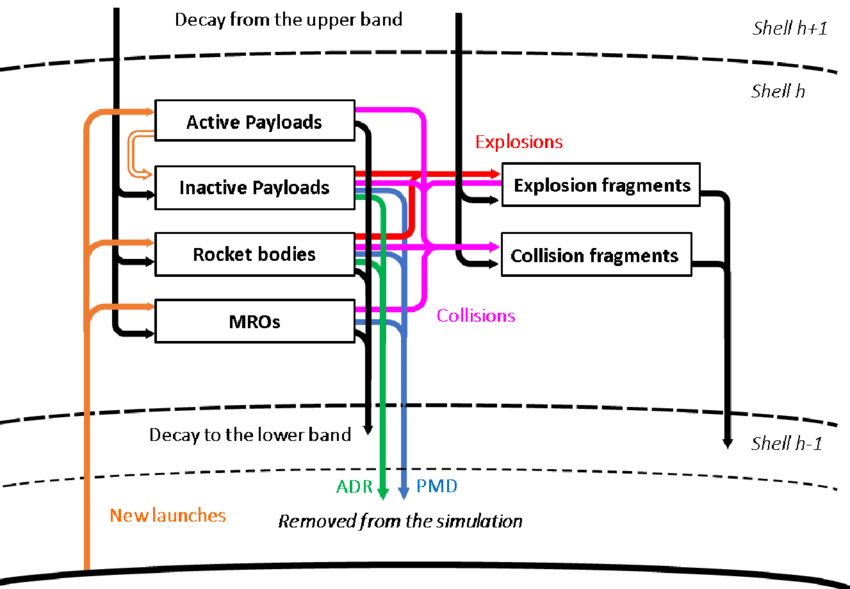
\includegraphics[width=0.9\textwidth]{Images/mechanism.png}\caption{Source and sink mechanisms depicting an object's injection and removal from a specific altitude. \textit{Source: \cite{Somma 2019}}}
\label{mechanism} 
\end{figure}

The total population of objects $N_T$ at every discrete time $t_k$ in a specific altitude shell $h$ can be found as:
\begin{equation} \label{total_population}
N_T(t_k, h) = N_{AP}(t_k, h) + N_{IP}(t_k, h) + N_{RB}(t_k, h) + N_{MR}(t_k, h) + N_{CO}(t_k, h) + N_{EX}(t_k, h),
\end{equation}
%these objects (N_{T}) etc. do not have the vector symbol - as it is shown in the paper of Somma- because it is just an array of values, but not a vector in mathematical or physical sense.

where the subscripts $AP$, $IP$, $RB$, $MR$, $CO$, and $EX$ refer to the objects of the following categories respectively: active payloads, inactive payloads, rocket bodies, mission related objects, collision and explosion \cite{Somma 2019}.

\pagebreak
In a similar manner, the derivative of the total population in each altitude shell can be found as:
\begin{equation}\label{derivative}
\dot{N}_T(t_k, h) = \dot{N}_{AP}(t_k, h) + \dot{N}_{IP}(t_k, h) + \dot{N}_{RB}(t_k, h) + \dot{N}_{MR}(t_k, h) + \dot{N}_{CO}(t_k, h) + \dot{N}_{EX}(t_k, h).
\end{equation}

Hence, the total population of the objects in any discrete time $t_k$ can be predicted using:
\begin{equation}\label{future}
N(t_{k+1}) = N(t_k) + \dot{N}(t_k, N(t_k))\Delta t.
\end{equation}

It can be concluded that if the derivative of the total population (\ref{derivative}) is positive then the objects being added outnumber the objects being removed, which leads eventually to congestion in those altitude regions of the outer space.

\bigskip
%There is a big problem especially in LEO
The above mentioned issue of the growing numbers of orbiting objects is mainly encountered in LEO. To be more exact, approximately 75\% of all cataloged objects are located in LEO, which results in several negative effects. Not only the risk of collision becomes bigger, but also the safety of human spaceflight is at risk, since ISS operated and performs in the LEO altitudes (\textasciitilde 350-400km) \cite{Kramer 2002}. The effect of this issue in the outer space was also noted by the CEO of a launch company mentioning that it becomes harder to find a path for rockets to launch new satellites \cite{crowded}.


\bigskip
\subsection{The reasons behind the growing number of objects in space}
\bigskip
%Reason why it happens/ Causes
The reasons behind the increase of the objects in space are manifold. Firstly, one root cause is the incremental number of launched objects, which is also highly connected to the free market, the commercial activities and the free competition between the private corporations. %(no trading restrictions)
One argument to launch more satellites by the \textit{Planet} company is that the commercial market has opened up since the daily revisits have been increased with the newly launched satellites and the offered resolution is higher. As a direct result, there is more demand as the costumers show greater interest, which is cited as a good reason to launch more objects \cite{CNBC}.

Even though the risk of collision is one of the side effects of this issue, in the event of an actual impact, the particles being created will definitely deteriorate the situation. This is in fact the vicious circle predicted by NASA's scientist Kessler. (Chapter \ref{chap:1.1}) Thus, as a second reason of the growing number of objects in space, the accidental break-ups can be mentioned. The first accidental collision between two intact satellites, which took place in 2009 at LEO, is undoubtedly a benchmark in space history. The number of debris left behind from this collision between the US \textit{Iridium-33} and the Russian \textit{Kosmos-2252} was more than 2,300 pieces with average size of 12.5cm and average mass 1.1kg \cite{Kelso 2009}. This impact is an indication that a collisional cascading might happen soon, if action is not taken.
%Between the US commercial non-operational Iridium-33 and the Russian military Kosmos-2251.

Another reason behind the increase of the objects in space is the satellite interceptions by surface-launched missiles. The anti-satellite tests are weapons, which not only aim at destroying satellites, but also their action creates uncountable space debris. As an example, in 2007, the intentional destruction of the chinese \textit{FengYun-1C} satellite doubled the amount of debris at an altitude of about 800 km, leading to a 30\% increase in the total population of debris at that time \cite{Anti-satellite}. Last but not least, the fact that there is lack of legally binding space traffic regulations, and mitigation guidelines, which are under international law, such problem is difficult to be handled.

\bigskip
\subsection{Negative effects \& temporary ways of collision avoidance}
\bigskip

Some of the negative effects of this crucial issue has already been emerged as discussed above, whereas some others are looming. The number of launched objects and the number of space debris is proportional to the likelihood of impact between two objects/ particles. In other words, when the number of objects in space increases, the risk of collision is higher. More specifically, after the first accidental aforementioned collision in 2009, the remote sensing satellites \textit{ERS-2} and \textit{Envisat} due to their proximity to the region of impact, have increased their risk of a secondary catastrophic collision by almost a factor 2 \cite{Klinkrad 2009}.

Another possible aftermath of the problem is linked to the deterioration of socio-economic conditions. Important services from space could be seriously affected in a negative sense or even be lost. Examples of such services could be weather forecasting, emergency management, as well as climate monitoring. Additionally, space-based communications and internet could be affected, resulting in a required disruption of the communication and transactions globally \cite{Undseth}.

\bigskip

The potential collision risk has led to find different other ways of mitigation. These are the creation of shields for protecting satellites from space debris, the need of surveillance and tracking of the orbiting objects, and the replacement of missions altogether to be equipped with the latest technology and to be able to maneuver if needed. Even though these measures had proved to be helpful, their operation do not solve the root of the problem.


\bigskip
\section{Mitigation principles of the growing number of orbiting objects}
\label{chap:mitigation}
\bigskip

\bigskip
\subsection{Taking action}
\bigskip

\subsubsection{Debris monitoring}
There are multiple ways towards reducing the creation of new objects in space. %confronting a problem
To begin with, the methods, which help towards the avoidance of collisions between the already launched satellites are the following. One approach is to track debris by using ground-based systems. Objects larger than 10cm in LEO and larger than 1m in GEO can be tracked \cite{Kramer 2002}. However, according to a recent study by the University of Warwick and the Defence Science and Technology Laboratory in the UK was found that more than 75\% of the objects that can be observed and that are bigger than 1m in GEO, could not be classified. It is absolutely urgent to continue observing the space debris in the GEO region in order to understand better what is the current situation before launching more objects \cite{Blake}. %Article in which I found it: https://newatlas.com/space/orbital-space-debris-threat-active-satellites/
 Smaller objects than the aforementioned sizes, not to mention objects in the mm scale, are difficult to be detected due to the sensitivity limits of the instruments, such as radars and telescopes.

\bigskip
\subsubsection{Collision avoidance}
Another way of dealing with the problem, which requires more effort, time and bears extra costs, is the method of collision avoidance messages and subsequently the action of maneuvering a satellite. In case there is an estimation of a possible collision with at least one of the involved objects being operational, maneuvering is the instinctive reaction of the satellite operators.

\bigskip
\subsubsection{Active space debris removal}
In a similar manner, a method, which will have a great impact on reducing the risk of collision especially with the big, non-operational satellites that are still orbiting Earth, such as \textit{Envisat}, is the active space debris removal. There are many other ways of space debris removal, such as the use of robotic arm, clamping mechanism, net, magnets, foam or even by using a collision with small relative velocity \cite{active, takeichi}. Some of the projects working in this direction is the \textit{ClearSpace} by ESA and the \textit{RemoveDEBRIS} by EU and University of Surrey.

\bigskip
\subsubsection{Deorbiting methods}
Several ways of deorbiting can also help into mitigating the issue of the growing numbers of objects in space. The uncontrolled reentry is one of them, which occurs when the satellite is sufficiently low (e.g. at about 600 km, the remaining lifetime may be about 30 years) to be affected by atmospheric drag, a process referred to as natural decay. This way of uncontrolled reentry is proportional to the ballistic coefficient, which is the effective drag area divided by the mass. Thus, in case of having a satellite with a high mass-to-area ratio, the decay is longer as compared to the decay of a satellite with a lower one. Although this method is a popular choice of disposing an object and thus not occupying space in an orbit slot, it still poses a threat. The reason behind is that the satellite passes unguided through lower altitudes and potentially keeps crossing orbital paths of other satellites for many years. On the other hand, there is the controlled reentry, which is a deorbiting option when the satellite is located approximately at 800 to 1,000km and the ground risk is above $10^{-4}$. Then, in this case the satellite is targeted to come down over the ocean and usually the south pacific with the use of thrusters. Another way of deorbiting, which was developed recently in the Chukyo University is by using drag force intensifier applying charged membrane \cite{muranaka}.


\bigskip
%A method, which prevents the further acting of deorbiting after the end of life of a LEO satellite is its placement to a MELVOs orbit (Moderately Elliptical Very Low Orbits) instead of a LEO one.
\subsubsection{The benefits of MELVO orbit}
A convenient method, which has been prepared and programmed for the deorbit of the satellite without further action after the end of life due to the orbit selection, is the following. Instead of placing a future LEO satellite in a LEO orbit, it is placed in a MELVOs orbit (Moderately Elliptical Very Low Orbits). The characteristics of a MELVO orbit is that the perigee and apogee are in a lower altitudes of 300 and 500km respectively and the eccentricity is between 0.015 and 0.030. Some of the advantages of this method is that when the orbit maintenance stops, the debris population can decay in this altitude and reenter the atmosphere in a short time, due the elliptical shape of the orbit. As a reference, from a circular orbit of 300km, it reenters the atmosphere in about 23 days at solar maximum and 70 days at solar minimum. Also, if there is a failure in the orbit maintenance burns, the orbit will turn into a circular one without loss of delta V. Another positive aspect of this idea is that since the perigee has low altitude, there is a better resolution on Earth and also reduced orbital debris issues, both in terms of collision probability and contribution to the long term debris problem \cite{Kramer 2002}. On the other hand, the disadvantages of this concept are that for station-keeping purposes delta V is required, the coverage is reduced compared to a LEO orbit and that it has a reduced design life. Nevertheless, it has potentially lower cost per year.



\bigskip
\subsection{Raising consciousness}
\bigskip

Several important steps have been made towards raising the consciousness about the growing numbers of objects in space, as well as the enactment of rules regarding the carrying capacity and orbit allocation. The most significant milestones that showed an international cooperation at a technical level are the following.

\bigskip
\subsubsection{First space debris mitigation guidelines}
\bigskip

In 1993 the \textit{Inter-Agency Space Debris Coordination Committee} (IADC) was founded. Its goal is to coordinate the efforts among the various space agencies that are involved and structure a plan for dealing with the debris orbiting the Earth. Some years later, in 2002 IADC published for the first time a report about Space Debris Mitigation Guidelines \cite{UNOOSA}. %The space debris mitigation was performed in 2002 by IADC and presented at UNCOPUOUS in 2003.
These guidelines were presented at the \textit{United Nations Committee on the Peaceful Uses of Outer Space} (UNCOPUOUS), which is a committee established by \textit{United Nations Office for Outer Space Affairs} (UNOOSA) \cite{IADC 2007}. In 2003 another group focused on similar goals was created – the \textit{Orbital Debris Co-ordination Working Group} (ODCWG). It was established by unanimous agreement of \textit{International Organization for Standardization} (ISO) \cite{Klinkrad 2006}.
%The two main groups that work towards these goal are the UNCOPUOUS and the ODCWG.

The first five mitigation guidelines, which were presented at the UNCOPUOUS in 2003, are related to the following concepts: prevention of the release of a mission related object, implementation of collision avoidance measures, prevention of explosions by releasing stored energy, disposal, passivation and limitation of the on-ground risk due to re-entry. Some other guidelines for the current debris mitigation are: the avoidance of intentional generation of debris, such as anti-satellite tests, as well as the 25-year deorbit rule for the LEO missions. As it was mentioned in the ESA's latest Space Debris Environment Report, less than 60\% of the LEO satellites comply to these guidelines \cite{ESA 2020}. %(from http://www.esa.int/Safety_Security/Space_Debris/The_cost_of_space_debris)

Even though there are national and international mitigation measures, the compliance is insufficient to stabilize the orbital environment. For this reason, it was investigated that by reducing the residual lifetime from 25 to 5 years we could prevent the increase of inactive population and thus the prevention of collision fragments. The commercial operators should commit to design objects with lower residual life. Thus, the satellite deorbit reliability will be maximized \cite{Somma 2019}.

The aforementioned Space Debris Mitigation Guidelines are applicable not only to mission planning and designing new spacecraft, but also to the existing orbiting objects if possible. The implementation of those guidelines is highly recommended, however it is a voluntarily action due to the fact that they are not legally binding under international law \cite{UNOOSA}.

% NO GUIDELINES SINCE 1967:
%The 1967 Outer Space Treaty, which remains the primary international document regulating activity in outer space, was agreed to at a time when only two governments were going to space. Now that more countries and commercial companies are also in the business of spaceflight, regulators are faced with a Catch-22: They don't want to create a lawless environment, but they're reticent to impose new rules for fear that other countries may become more dominant in space.
%Recent attempts to update rules on the international stage have been "incredibly inspiring, but also incredibly depressing," Beck said. Because even though countries were willing to come to the table, nothing has actually been agreed upon since the 1970s. Source: https://edition.cnn.com/2020/10/07/business/rocket-lab-debris-launch-traffic-scn/index.html

\bigskip
\subsubsection{Comprehensive tool for space debris mitigation guidelines}
\bigskip
One of the difficulties that a mission faces in the designing phase is the compliance to the space debris mitigation guidelines. The reason that lies behind is the existence of various regulations from different entities, such as UN, EU, ECSS, ISO and others. In order to be tackled, ESA is currently developing a software the so-called Debris Mitigation Framework (DMF), in which all the necessary information and tools regarding the requirements, standards and guidelines are collected. The software is based on the very well known DRAMA and MASTER tools. So, DMF is the link between all the needed information about a mission and the space debris mitigation needs, which has been specified by the user \cite{Braun}.

\bigskip
\subsubsection{Space sustainability rating}
\bigskip
%SPACE SUSTAINABILITY RATING - HOW WELL AN INDIVIDUAL SATELLITE FOLLOWS THE GUIDELINES.
The fact that the existing international guidelines are not enforceable and the derived standards are not always followed, has led the \textit{World Economic Forum} (WEF) to select a consortium of companies, universities and agencies in order to create a system for rating the sustainability of space systems \cite{Space sustainability}. %Source: https://www.weforum.org/projects/space-sustainability-rating
In particular, this project is consisted of an international and multidisciplinary team and the main collaborating entities are the \textit{European Space Agency} (ESA), \textit{Massachusetts Institute of Technology} (MIT), \textit{University of Texas at Austin} and \textit{Bryce Space and Technology}. The so called Space Sustainability Rating (SSR) concept has the goal of encouraging a responsible behavior in space through increasing the transparency of organization's debris mitigation efforts.
%Francesca Letzia and Stijn Lemmens (from ESA) are working for that. Another idea would be also to have the concept of added-value incorportated into that rating. But still it seems very difficult - so it is not part of the parameters.
%The other side of the insurance companies say: If one constellation has a good rating, then the insurer (insurance company) will make a discount. But at the same time this will probably affect the requests for insurance claims on satellites (since the rating is good and thus the risk as well of collision is small - the satellite companies might not want to be insured). *These are just guesses...!*

In order to ensure the long-term sustainability of space, a measurement for every individual satellite or constellation will be carried out, which will show the degree of commitment to the guidelines. 
%The SSR will give a score related to debris mitigation and alignment with international guidelines. (I said it with other words.)
The calculation of this score will take into account both quantitative and qualitative parameters. Some determinant parameters are each satellite's design and physical parameters, the economic viability of the satellite's operator (relevant example of \textit{OneWeb} \cite{Oneweb_bankruptcy, Cadman}), % In case, a company declares bankruptcy, as OneWeb (UK) did, many already launched satellites are doomed to stay in LEO occupying space in that area and increasing the risk of collision when they will be become non-operational. (There are now in orbit around 70 OneWeb satellites). Chinese investors are interested into buying the company. The United States and other Western nations are not keen on the idea of seeing OneWeb slip into "adversarial hands.") British government and Indian mobile network operator Bharti Global placed the winning bid to acquire OneWeb (1 billion$).
how trackable the satellite is, estimations concerning potential collisions and the satellite's disposal at the end of its life. 

Currently there are so many different definitions of space sustainability and this term needs to be shaped and generally accepted. Nevertheless, this level of sustainability of a mission will be publicly available by placing emphasis on the debris mitigation approach and by giving a positive incentive to satellite operators to increase their responsible behavior and to improve their ratings. An initial beta version of this rating system is going to be released at the end of 2020/ beginning of 2021 \cite{Space sustainability}.
%Source: https://www.weforum.org/projects/space-sustainability-rating

\bigskip
\subsubsection{Concept of orbital capacity}
\bigskip

The concept of orbital capacity was formulated in order to estimate the global evolution of the space environment. Every orbital plane has a certain capacity, which should be taken into account when a future satellite constellation is going to be launched. Towards this goal, the calculation of the Space Debris Index is essential. It is based on the collision risk of operational satellites and the collision effect, as well as the explosion probability and effect. This index can be applied to both single objects and to the whole environment. As a direct consequence, when there is more capacity, then the reliability, which is connected to the Post Mission Disposal success rate, is low. The concept of orbital capacity will be used to sharpen the current space debris implementation guidelines \cite{Letizia 2019}.

In this way, along with the concept of "Space Sustainability Rating" (SSR), the concept of "Space Traffic Footprint" will be created. It will include data on the size and location of an object, how crowded the orbital area is, what already exists there and if a satellite is maneuverable and trackable \cite{Space sustainability}.
%Source: https://phys.org/news/2019-05-space-sustainability-aims-amount-debris.html

\bigskip
Some other methods that can help into mitigating the issue related to the growing numbers of objects in space are the following. The concept of added value is based on the estimation of the characteristics of a satellite or a constellation before they are launched. In this way, the launching of the missions can be prioritized based on the added value it is expected to provide to the society. Another idea of dealing with the aforementioned issue is the concept of the cooperation between the entities towards sharing common resources. More details about those concepts can be found in the following section (Section \ref{section}).


\bigskip
\section{Mitigation concepts encouraged by the current work}
\label{section}
\bigskip

\subsection{Estimation of added value}
\bigskip
%ESTIMATION OF ADDED VALUE
As it was mentioned in Chapter \ref{chap:scope}, the goal of this thesis is to give the incentives for the formation of rules which will be based on the added value that a new satellite offers. As an example towards this direction is the report of the independent consultancy, London Economics (LE), which is working in the space sector, regarding the value of the EO capabilities offered by satellites to the UK government \cite{Value UK}. In this case the value is determined based on multiple parameters such as the operational cost saving, the exceptional cost avoidance, better policy decisions and the benefits that the government, the economy and the society gain from the offered EO satellite capabilities. This study can be a great approach and can serve as an example to other nations and institutes towards prioritizing the missions based on their potential value to the society.

In the current work, the developed application offers the opportunity to a user to find out how many satellites have the same characteristics, such as same sensors, similar revisit time, common field of utilization, such as Environmental monitoring - etc.

\bigskip
\subsection{Cooperation between entities towards sharing resources}
\bigskip

A different way of mitigating the issue related to the growing numbers of objects in space, which is also connected to the aforementioned idea of added-value, is the concept of the cooperation between entities towards sharing common resources. As it has also been mentioned in the GEO (\textit{Group on Earth Observations}) summit in Tokyo, 2004, when the GEOSS (\textit{Global Earth Observation System of Systems}) was created, in order to have a societal benefit of Earth Observation, data sharing is necessary \cite{Kramer 2002}. %Krmaer p.39
The Argentinian and the Italian space agency, CONAE and ASI respectively, have showed interest in this direction. They have the vision of integrating the two national systems by using their EO constellations, \textit{SAOCOM} of Argentina and \textit{Cosmos-SkyMed} of Italy in order to generate information for the sector of Emergency Management on environmental issues \cite{Cosmos}.  %SAR sensors

Another example is the group \textit{BRICS} consisted of the states Brazil, Russia, India, China and South Africa, which will join their forces towards a mission regarding natural resources and disaster management. They will use already existing/ orbiting Sun-Synchronous Remote Sensing satellite \cite{BRICS}. An initiative was also taken from UNOOSA under the name of \hspace{1mm} “Access to Space for All”, which has the goal of connecting and creating necessary conditions for cooperation between the established space actors in order to achieve the SDGs (Sustainable Development Goals) \cite{UNOOSA}.
%Other links related to the symposium in 2020: https://www.unoosa.org/documents/pdf/copuos/stsc/2020/acces2space4allprogE.pdf + https://www.unoosa.org/oosa/en/ourwork/copuos/stsc/2020/unoosa-symposium.html

In the same manner, the National Reconnaissance Office (NRO) of USA searches for commercial companies in order to support the US government missions. The procedure that is followed is the inspection of each company's current and planned capabilities, as they want to have more than one collaborator/ provider. This is noteworthy, since not only this request gives the incentives for collaboration among companies, but also the creation of a state of monopoly in space is certainly undesirable \cite{NRO}.

A more recent example of entities which have cooperated with each other towards a common goal is between ESA and NASA in order to measure Antarctic sea-ice. This joint-campaign is known as Cryo2Ice with the following satellites participating, CryoSat-2 (ESA) and ICESat-2 (NASA). This cooperation will involve orbit synchronization, since the number of coincident observations observed by the two satellites needs to be increased. The instruments that the two satellites carry on-board are different. More specifically, NASA's IceSat-2 has laser, which measures the distance to the Earth's surface and thus the height of objects. On the other hand, ESA's Cryosat-2 uses radar, which is penetrating more deeply to the snow than laser before bouncing back. The idea for this tandem mission observing the polar regions came from the fact that the advantages of both sensors will result in more reliable outcomes \cite{Cryo2ice_news, Cryo2ice}.
%ESA (CryoSat-2, radar ~720km) and NASA (ICESat-2, laser  ~500km). Cryosat-2 changed orbit by raising the altitude in approximately one kilometer. "Icesat is quite a bit below us so we can't go down to meet them, but by going up we find this incredible resonant orbit in which for every 19 orbits for us and 20 orbits for them - we will meet at the poles within a certain time lag. Basically, every 1.5 days, we meet over the poles within a few hours of each other and that means we can observe the same ice almost simultaneously."

Additionally, another cooperation that has been actualized is between ESA's Copernicus Sentinel-5P and GHGSat’s Claire. The goal is to map a range of atmospheric gases around the globe every 24 hours. Collectively the different sensors of those two satellites can identify significant methane leaks, which can lead to better monitoring of the climate change \cite{cooperation}. %The same will happen with the next satellite "Iris".

% Cooperation between companies: Planet and Copernicus encourage people to use jointly their data (there is also the challenge “See change, change the world”) --> I don't think that it has the character of mitigating the problem of overpopulation etc. Or that the cooperate for this reason.

\bigskip
\section{Orbit and mission type focused in the current work}
\bigskip

As it was mentioned in Chapter \ref{chap:scope}, the main goal of this master thesis is the development of an application, which is focused on Low Earth Orbits in the field of Earth Observation. For this reason, the section below is comprised of the main attributes and important parameters of those two sectors.

\bigskip
\subsection{Low Earth Orbits}
\bigskip

\subsubsection{General characteristics}
\bigskip
Low Earth Orbits (LEO) are placed in the closest region above Earth's surface. Their altitude ranges from 200 to 2000 km, which leads to a limited swath area on the surface of the globe. They are characterized by short orbital periods between 88-127 min and thus many revolutions per day. Their orbital velocities are high, around 7-8 km/s with regards to an observer on Earth and inclinations between zero and 180 degrees \cite{Campbell}.

The LEO is also a favorable spot for placing satellites for various reasons. It's proximity to Earth makes it possible to launch even CubeSats to naturally decay and burn up in Earth's atmosphere within a few years. Specifically in the recent years more and more small satellites and/or CubeSats are placed in LEO and in large constellations (Fig. \ref{launch_traffic_LEO}). The need of proliferated constellations is also linked to the low altitude of the LEO region. Namely, for larger coverage, a satellite should be either placed in a higher altitude, or the mission should engage more satellites in order to compensate the smaller field of view that one satellite offers.

The main areas that LEO is used are for remote sensing, Earth observation, human spaceflight, climate, weather forecast, military, and others. 

\pagebreak
\subsubsection{LEO subcategories}
\bigskip

\begin{itemize}
\item Classification based on eccentricity
	\begin{itemize}
	\item Circular LEO: \\
	It is the most common and natural orbit for Earth Observation. The typical altitude ranges from 200 to 900 km with orbital periods of about 90-105 min.
	\end{itemize}
\item Classification based on inclination
	\begin{itemize}
	\item Equatorial or tropical orbit: \\
	The inclination of this orbit is zero or close to zero degrees. It provides close coverage of the tropical regions.
	\item Polar or near-polar orbit: \\
	In such an orbit the inclination is 90 degrees or near 90 degrees, but necessarily larger than 60 degrees. Therefore, this orbit passes above or nearly above the poles on each revolution. \\ % Their orbit which is basically north-south with conjunction with the Earth's rotation (west-east), allows them to cover most of the Earth's surface over a certain period of time.
	\\
	A polar orbit has definitely some advantages, as they were mentioned previously. However, the choice of a certain altitude is determinant. A lower altitude results in:
		\begin{itemize}
		\item a shorter orbital period,
		\item poorer coverage of the surface,
		\item stronger return of signals,
		\item better spatial resolution,
		\item and greater drag and shorter lifetime.
		\end{itemize}
	\item Polar sun-synchronous orbit: \\
	It is a special case of a near-polar orbit, which combines certain parameters in such a way that the satellite passes over a given area of the world at a constant local time of the day. This time is called local solar time.
	
	To begin with, an orbit like this is possible by the fact that the Earth is not a perfect sphere. It should move one degree per day in order to compensate for the Earth's revolution around the sun. Hence, this precession is responsible for the satellite's crossing of same areas at the same local solar time \cite{Meseguer, Kramer 2002}. This can be seen in the Figure \ref{sso}.
	
	However, the altitude and the inclination are also two determinant parameters that define such an orbit. A typical SSO orbit has altitude in the range of 400 to 1000 km and inclination in the range of 97 degrees to 100 degrees. Another characteristic is that the daily rotation of the orbital satellite plane with respect to the equatorial plane is identical to the mean motion of the Earth around the sun. In other words, the orbital period is an integral multiple of the sidereal day \cite{Campbell}, and this leads to a repeating groundtrack.\\ %In particular, some satellites repeat their groundtrack in some days, which is called shallow resonance, and others in some years, namely deep resonance.\\
	% It is then clear that a SSO is not fixed in space. In other words, the plane of a satellite, which is in a sun-synchronous orbit (SSO) has always the same relation to the sun.
	%Since the Earth makes one revolution around the sun per year, which is 360 degrees, the rate of change of the sun's right ascension is calculated.	
	%0.9856473°/solar day. > This is the required rate of precession of \Omega. 
	%The inclination of the orbit (for circular orbits) and altitudes between 400 km and 1000 km, is in the range of 97° to 99°. Therefore, they are also quasi polar orbits, which allow the whole surface of the Earth to be covered, even passing several times a day over the same point. + Their altitudes usually range from 700 to 800 km, with orbital periods of 98 to 102 minutes. (NOT SURE)
	% In case you want to put a figure showing the relationship that the inclination and the altitude (time period) need to have, check: "2019_Joint_Agency_Commercial_Imagery_Evaluation.pdf" is in the folder of check in Literature p.29.
	\\
	This is a great benefit especially for the Earth observation satellites, since the area of interest can be monitored throughout the year with similar illumination conditions and the changes can be easier detected. An additional advantage is that there is no need of correction due to difference illumination conditions in case the purpose of a project is to create the mosaic from adjacent images. \\
	\\
	It is also worth mentioning that in the case of a sun-synchronous orbit with an optical or else passive sensor, the images that were captured in the sunlit side of the Earth are of great interest. In the case of active sensors, which provide their own illumination or passive sensors that record emitted radiation, the outcome of both sunlit and shadowed side of the Earth is useful.	A satellite's orbit can be designed in a way so that the sun is in a certain position whenever the satellite passes from the area of interest. This position can also be associated with the mission objective. For example, if the mission is focused on urban planning and street detection, a very low angle of the sun in the sky will result in many shadowed areas causing difficulties in achieving the mission's goal. Another example is of an orbit focused on monitoring glaciers. In such case, the sun ideally should not be at the highest point in the sky, since surfaces like ice have high reflectance, which might cause saturation. 
		%Most of the times the satellite is designed in order to acquire these outcomes from the descending pass of the orbit, which corresponds to the north-south movement of the satellite. This happens especially when the area of interest is in the northern hemisphere. Additionally, the position of the sun should be neither at a very low angle in the sky, since it would result in many shadowed areas, nor at the highest point in the sky, due to the saturation that surfaces like ice, which have high reflectance, might cause. So, one compromising option is to acquire images at some time in between; in the mid-morning. % https://www.nrcan.gc.ca/maps-tools-publications/satellite-imagery-air-photos/remote-sensing-tutorials/satellites-sensors/satellite-characteristics-orbits-and-swaths/9283
	 \cite{Campbell}.\\
	\\
	As it was mentioned, the benefits of the near polar and sun-synchronous orbits are very significant especially for the missions, which focus on Earth Observation. This is also depicted in the Figure \ref{inclination-satellites}, in which the distribution of the existing Earth satellite orbits by inclination is shown. The 30\% of the cataloged satellites are in a sun-synchronous orbit.
	\end{itemize}
\end{itemize}

\begin{figure}
\centering
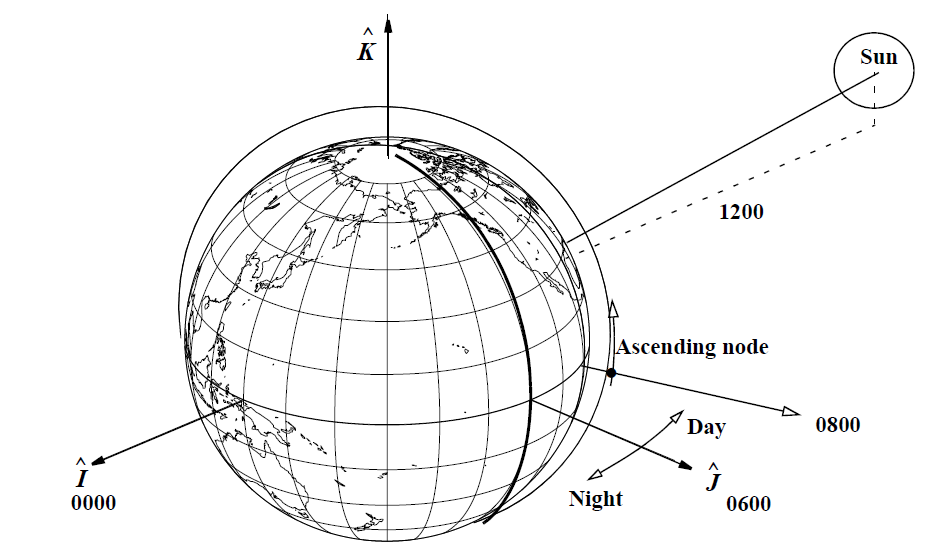
\includegraphics[width=0.9\textwidth]{Images/sso.png}\caption{Geometry for sun-synchronous orbits. The satellite shown reaches the ascending node at 8:00 AM local time as the orbit's name denotes; 0800. \textit{Source: \cite{Vallado}}}
\label{sso} 
\end{figure}

\begin{figure}
\centering
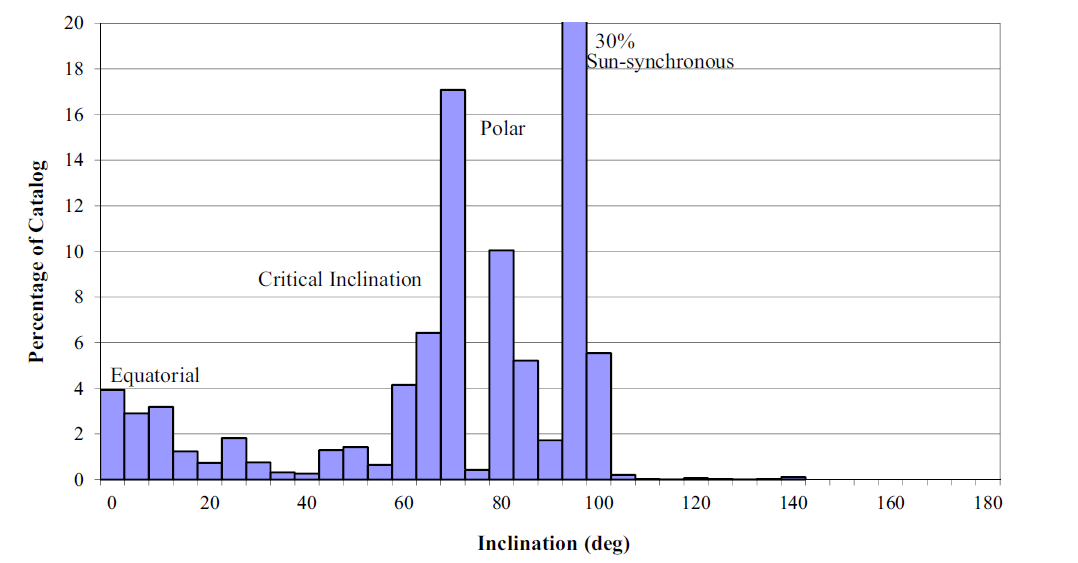
\includegraphics[width=0.9\textwidth]{Images/inclination-satellites.png}\caption{Distribution of existing Earth satellite orbits by inclination as of December 2012. The large concentration of satellites are in the polar and sun-synchronous regions. \textit{Source: \cite{Vallado}}}
\label{inclination-satellites} 
\end{figure}

\bigskip
\subsubsection{Critical regions of LEO}
\bigskip

The total number of operating satellites in outer Space is 2,787 with 2,032 being in LEO as of 31.07.2020 \cite{UCS}. Undoubtedly, LEO is the most crowded region orbiting Earth, which is declared as protected region by IADC (Inter-Agency Space Debris Coordination Committee) \cite{IADC 2007}. In the recent years, many studies have been conducted into detecting the highly populated regions in LEO.

Even though the boundaries of the LEO region are located from 200 to 2000 km above the Earth's surface, there are three critical regions according to Kramer \cite{Kramer 2002}, which are the following:
\begin{itemize}
\item The first critical region is at the altitude 750-850 km, at which the spatial density is increased because of the debris' population. It is characterized as critical, because objects need hundreds of years in order to decay and re-enter the atmosphere.
\item The second critical region is at the altitude 900-1000 km, at which there is a high number of massive objects. Drag is also not sufficient in order to help objects decay and thus the spatial density increases over time.
\item The third critical region is at the altitude 1100-1300 km. At this region the effect of drag is negligible, which means that any additional object builds up the orbital population.
\end{itemize}

A more recent study was carried out by Somma et al. [2019], which simulated the population of the LEO from 2009 till 2209, based on the population statistics of the period 2009-2016. As it can be seen in the Figure \ref{Somma} there are three alarming regions, confirming the \cite{Kramer 2002} study as the two findings of the studies are similar.
\begin{itemize}
\item The major density peak region is found at the altitude 750-800 km.
\item In addition, the second high density peak region is at the altitude of 900-1050 km. It can also be noticed that the two aforementioned zones tend to get closer over time almost merging with each other (Figure \ref{Somma}).
\item Last but not least, there is a third region with high density numbers at 1400-1550 km.
\end{itemize} 

\begin{figure}
\centering
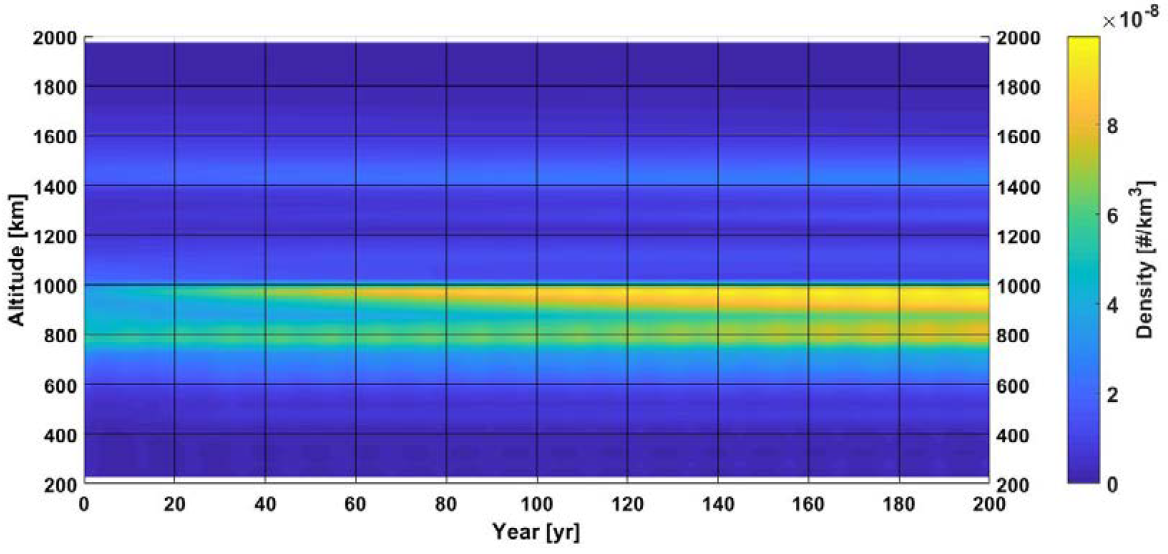
\includegraphics[width=0.9\textwidth]{Images/Somma.png}\caption{The evolution of the total spatial density in the LEO region. \textit{Source: \cite{Somma 2019}}}
\label{Somma} 
\end{figure}

Those peaks in the density prelude higher collision rates, which can generate more collision fragments. As it seems nowadays, the future large constellations will be placed around these altitudes, which makes these regions even more alarming \cite{Somma 2019}.

Another simulation of the debris population in LEO generated by ESA's MASTER-2009 tool was carried out by Crisp et al. [2020]. It was executed over the period 2020-2055 based on a business-as-usual scenario regarding the debris mitigation. As it can be seen in Figure \ref{crisp1}, there are two major peak density regions in LEO. The first one is approximately from 700-1000 km and the second one is from 1400-1500 km. A similar conclusion can be reached from the averaged spatial density in LEO (Figure \ref{crisp2}). The fact that in this study the recent mega-constellations that are soon-to-be launched, e.g. from SpaceX Starlink, OneWeb, were not included, makes the situation even more alarming \cite{Crisp 2020}.

\begin{figure}[!htb]
\centering
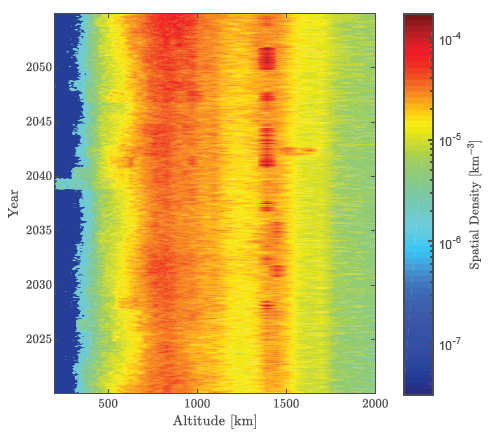
\includegraphics[width=0.9\textwidth]{Images/crisp1.png}\caption{Simulated LEO debris population (spatial density) over the period 2020-2055. Generated using ESA's MASTER-2009 tool. \textit{Source: \cite{Crisp 2020}}}
\label{crisp1} 
\end{figure}

\begin{figure}[!htb]
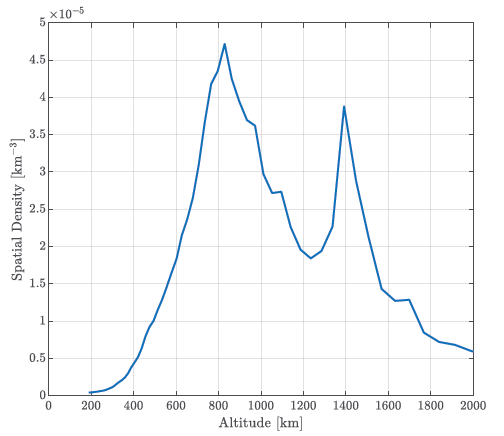
\includegraphics[width=0.9\textwidth]{Images/crisp2.png}\caption{Average spatial density for LEO altitudes over the period 2020-2055. \textit{Source: \cite{Crisp 2020}}}
\label{crisp2} 
\end{figure}

\bigskip
\subsection{Earth Observation}
\label{EO}
\bigskip

The type of satellites, on which this current master thesis focuses, is the Earth Observation satellites. Earth Observation (EO) is the process of acquiring observations, data, or measurements of the Earth remotely. One of the most common form of data that can be acquired from this field is the digital imagery and for this reason the main types of EO imagery will be described below. \cite{ESA EO}

\bigskip
\subsubsection{Passive imagery}
\bigskip

Passive imagery detects the electromagnetic emissions from particles of the Earth's surface and atmosphere. Usually depends on the day-night cycle, since these emissions are most of the times the result of reflected sunlight. According to the wavelength spectrum that the sensor can cover, the passive imagery is divided into the following categories:
\begin{itemize}
\item Panchromatic: \\
The images of this type detect and measure the light intensity in the full visible spectrum. However, the final product is displayed as shades of grey. Another domain, which can be captured by this product, is the thermal infrared (IR). In this case, the intensity of the image is correlated with the temperature of the object emitting that radiation.
\item Multi-spectral: \\
A multi-spectral image has usually measurements in 3 bands of the visible spectrum, centered around the blue, green and red wavelengths, which is also called "natural colour". Since in this category several narrow bands of the electromagnetic spectrum are involved for the production of the image, the resolution of the image is lower than of a panchromatic image. Nevertheless, multi-spectral images are not restricted to the visible spectrum or the combinations of the wavelength bands.
\item Pan-sharpened: \\
Pan-sharpening is a numerical process, which produces a high resolution coloured images. Since a panchromatic image have a high spatial resolution and the respective multi-spectral image a high spectral resolution, their combination can lead to an improved version of both.
\item Hyper-spectral: \\
A hyper-spectral image measures the light intensity for a large number of contiguous narrow spectral bands for each pixel.
\item Microwave Radiometry: \\
In this field, the measurement of the atmospheric water vapour column and cloud liquid water content are the main objectives. This aims at the improvement of the radar altimeter signals.
\end{itemize}

\bigskip
\subsubsection{Active imagery}
\bigskip

On the contrary to passive imagery, active imagery systems transmit a specific electromagnetic signal, whose return can be useful into understanding more about the Earth's surface. There are several methods and types of signals in the active imagery, such as:
\begin{itemize}
\item Synthetic Aperture Radar (SAR): \\
SAR is the most common active sensor in the field of EO. Electromagnetic pulses are transmitted towards the Earth's surface, which are either reflected or scattered by the surface. The intensity of the return pulse, which is detected by the instrument's antenna, is used for the generation of the SAR imagery. The fact that the radar imaging does not depend on the illumination of the scene, or on the meteorological conditions, makes the radar imaging a sensor, which can be used in multiple situations.
\item Light Detection and Ranging (Lidar): \\
Similarly to SAR, Lidar is an active sensor using IR, visible, or UV wavelengths. The applications that it can be found useful are for the precise measurement of topographic features, profiling clouds, measuring winds, aerosols or other atmospheric components.
\item Radar Altimetry: \\
A sensor of radar altimeter uses very short electromagnetic pulses in order to measure the surface topography profile along the satellite track. It can be used for acquiring the ocean and land topography, the ice sheets or even mapping the sea floor.
\item Radar Scatterometry: \\
Radar scatterometer is a sensor with which the direction and the speed of the wind can be measured. This result can be produced based on the reflection or scattering effect produced while scanning the surface of the Earth. Finally, the measurements of the backscatter from the waves at the sea surface are necessary for calculating information regarding weather forecast, oceanography, as well as climate changes.
\end{itemize}


\bigskip
The main and most related categories of the Earth Observation to the current work, were previously described. There are many other parameters, which are related to the EO imagery, such as the spatial resolution, off-nadir angle, revisit time and others. In the Chapter \ref{chap:3}, all the involved parameters are extensively analyzed and discussed. 


%----------------------------------------------------------------
%Regarding the field of remote sensing: "The critical design goal then is to place the satellite in an orbit that is low enough to permit a relatively short orbital period while at the same time the orbit is high enough to permit observation of a wide enough swath so that during a single orbit the Earth will rotate by less than the scan swath of the satellite's instrumentation. By placing a satellite at an altitude of about 850 km, you get an orbital period of roughly 100 minutes. At this altitude, you can get true global coverage if the scan swath of the satellite's instrumentation is about 3000 km." ABOUT THE SSO: "The orbit, however, can be improved if the orbital plane is inclined slightly away from a true N-S orbit. In this case, the asymmetric gravitational pull of the Earth introduces a slow precession in the orbital plane. With a inclination of about 98.7 degrees, the orbit will precess at almost exactly the same rate that the Earth rotates around the sun. That means that the satellite's orbital plane will appear to be fixed with respect to the sun, or sun-synchronous. Due to the inclination away from N-S, these satellites do not go directly over the poles, but do get close enough to provide true global coverages from a single satellite. Since the orbit is aligned with respect to the sun, in fact, you get twice daily coverage of every portion of the globe." Source: https://ral.ucar.edu/~djohnson/satellite/coverage.html#polar

%GEO KIND OF SUB-CLASSES:
%  Geosynchronous orbit:  is one in which the satellite orbits at the same angular velocity as the Earth.
%  There is also Geostationary orbit, which is a circular (zero eccentricity), geosynchronous orbit with an inclination equal to zero (equatorial). A satellite placed in such an orbit would appear, to an observer on the surface of the earth, to remain stationary in the sky. The footprint eventually depends on the field of view. Geometrically, a satellite at geostationary altitude can see a footprint about 70 degrees north and south of the equator. The benefits of such positioned satellite are increasing  its popularity and thus, crowded areas are produced in space. (Example about the benefit: A single sensor placed at a longitude equal to the center of US, which can monitor the weather pattern of the entire country continuously. Similarly, a communications relay station placed at a longitude in the middle of the Atlantic or Pacific oceans could allow direct communications between countries on either side or ships upon the seas. There are many more uses!)
%Because Earth rotates at a constant angular rate, a geostationary satellite must move at a constant speed in its orbit.
%Considering the fact that the semimajor axis of a geostationary orbit is around 42,168km, then it is calculated that the higher latitude that a geostationary satellite can view is λmax =81.3deg --> cos(λmax)= R_E / r_GEO = 6378/42,164 ==> λmax = 81.3deg. (WHY 42,164 when i said semimajor axis 42,168km ?)
%Some advantages and  disadvantages of geostationary orbits for remote sensing are the following. The Advantages are that almost all of a hemisphere can be viewed simultaneously and that the time evolution of phenomena can be observed. The disadvantages are that accurate measurements are difficult because the satellite is so far from Earth and that the polar regions are only observed at an oblique angle (good coverage only up to ~60° latitude).
%(Source: Campbell BA, McCandless W (1996) Introduction to space sciences and spacecraft applications. Elsevier)
%    Molniya Orbits: A Molniya orbit is an elongated elliptical orbit at an inclination of 63.4° for which the argument of perigee is fixed. Because ω is fixed, the apogee stays at a given latitude. These are used for communications satellites by the former Soviet Union because geostationary satellites provide poor coverage of the high latitudes of the FSU. They have also been suggested for meteorological observations at high latitudes. The apogee (and slowest speed) is over the FSU, and the perigee (and fastest speed) is over the opposite side of the globe, so that the satellite spends most of its time over the FSU. It stays in the apogge for about 8 hours!